%!TEX program = xelatex
%%%%%%%%%%%%%%%%%%%%%%%这是导言部分的开始%%%%%%%%

%========= 导言部分声明文档的类型=================
\documentclass{article}

%=========导言部分可可以加载宏包=================
\usepackage{amsmath}                % 数学公式排版宏包
\usepackage{amssymb}                % 数学符号命令宏包
\usepackage{amsthm}                 % 数学定理宏包
\usepackage[UTF8]{ctex}             % 中文输入宏包
\usepackage[a4paper]{geometry}      % 页面设置宏包
\usepackage{setspace}               % 行间距宏包
\usepackage{graphicx}               % 图片宏包
\usepackage{listings}               % 代码宏包
\usepackage{color}					% 颜色宏包
\usepackage{xcolor}                 % 颜色处理宏包
\usepackage{float}                  % 浮动对象式样宏包
\usepackage{fontspec}
\usepackage{enumerate}				% 列举编号包

%=========页面设置==============================
\geometry{left=1cm,right=1cm,top=1cm,bottom=2cm}
\onehalfspacing
\setlength\parindent{0em}

%=========代码格式设置============================
\definecolor{dkgreen}{rgb}{0,0.6,0}
\definecolor{gray}{rgb}{0.5,0.5,0.5}
\definecolor{mauve}{rgb}{0.58,0,0.82}
% \setmonofont{Consolas}
\lstset{
	numbers = left, 	
	numberstyle = \color{gray}, 
	keywordstyle = \color{blue},
	commentstyle = \color{dkgreen}, 
	stringstyle = \color{mauve},
	basicstyle = \ttfamily,
	breaklines = true,
	frame = shadowbox, % 阴影效果
	rulesepcolor = \color{ red!20!green!20!blue!20} ,
	escapeinside = ``, % 英文分号中可写入中文
	xleftmargin = 2em,xrightmargin=2em, aboveskip=1em,
	framexleftmargin = 2em
} 

%=========导言部分可以定义标题信息===============
\title{组会报告}
\author{徐益}
\date{\today}
%%%%%%%%%%%%%%%%%%%%%%%这是导言部分的结束%%%%%%%%%

%%%%%%%%%%%%%%%%%%%%%%%这是正文部分的开始%%%%%%%%%
\begin{document}

%=========生成标题================================
\maketitle

%=========开始正文的输入==========================

%===========第一节=================
\section{工作内容}
1. 测试信道特性;

2. 根据SVN目录结构修改makefile;

%===========第一节=================
\section{测试信道特性}
\subsection{TA补偿}
\begin{figure}[H]
	\centering
	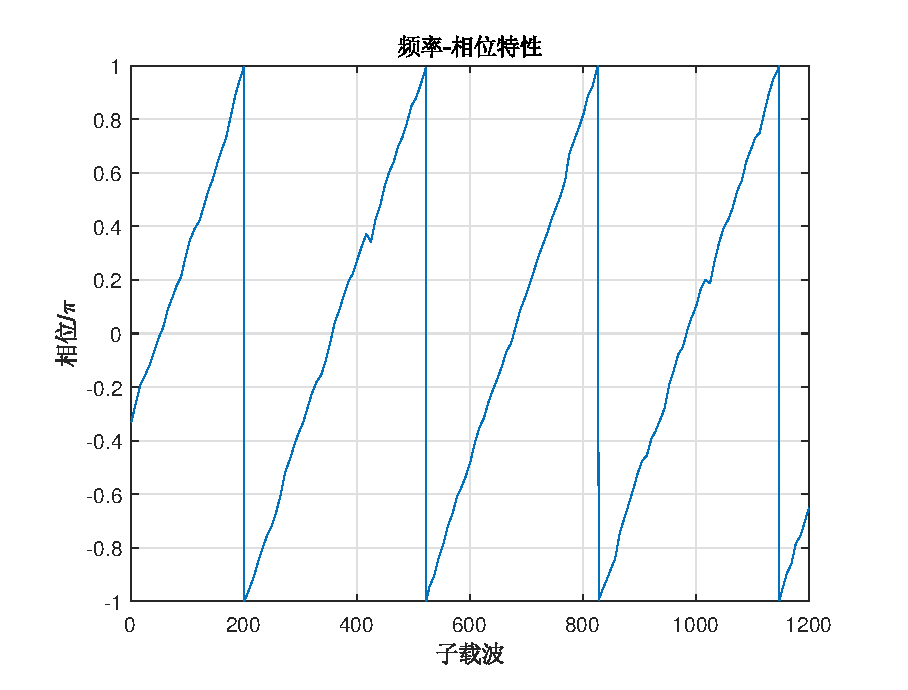
\includegraphics[width = .8\textwidth]{before.eps}
	\caption{原信号相频特性(测试TA=8)}
\end{figure}
\begin{figure}[H]
	\centering
	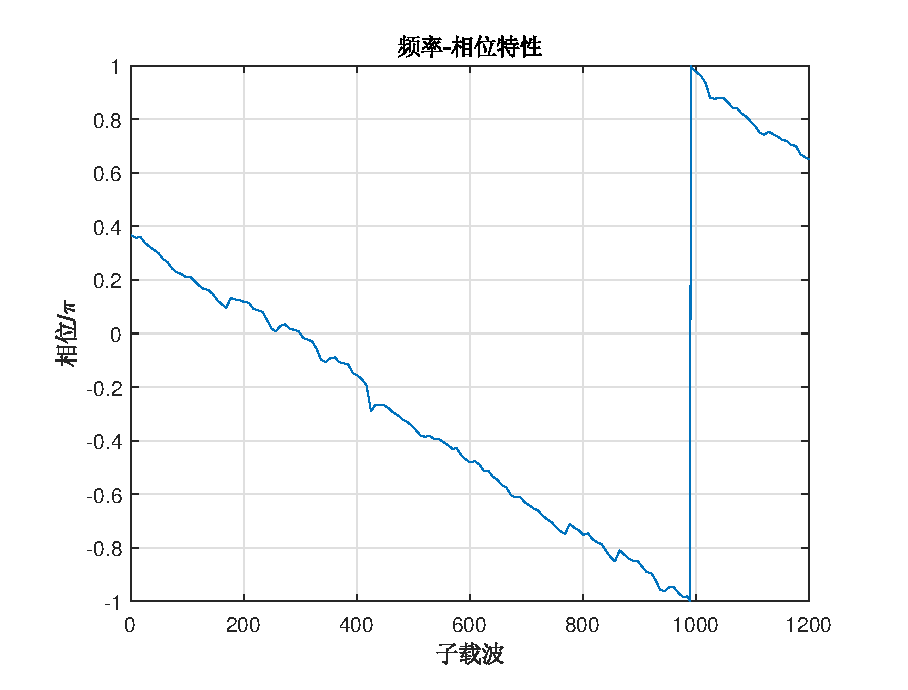
\includegraphics[width = .8\textwidth]{after.eps}
	\caption{TA补偿后的信号相频特性(测试TA=0)}
\end{figure}
\begin{figure}[H]
	\centering
	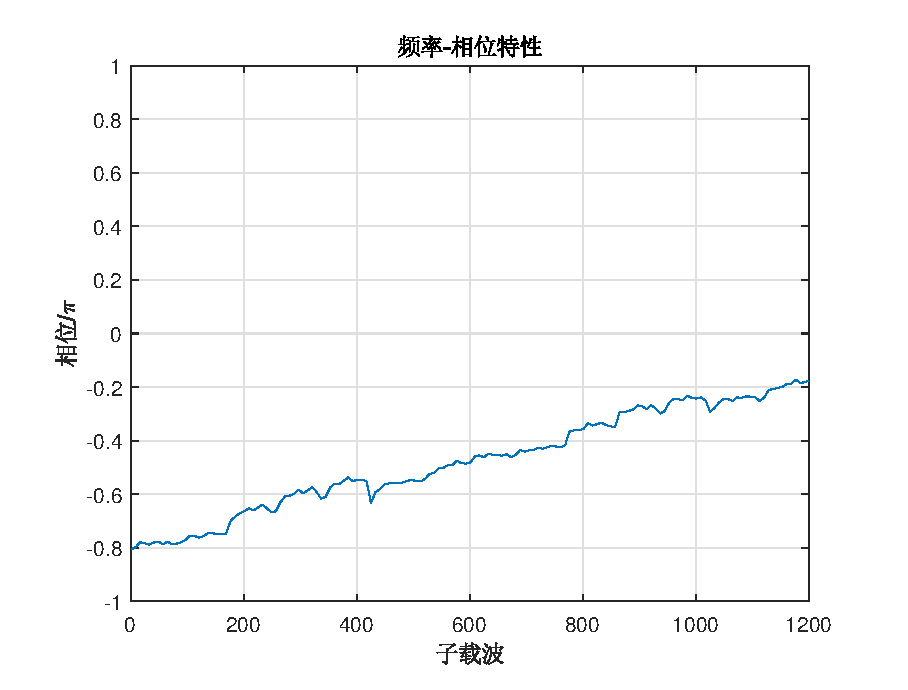
\includegraphics[width = .8\textwidth]{fp6.eps}
	\caption{TA补偿后的信号相频特性(测试TA=2)}
\end{figure}
\subsection{Zc序列发送测试}
\begin{figure}[H]
	\centering
	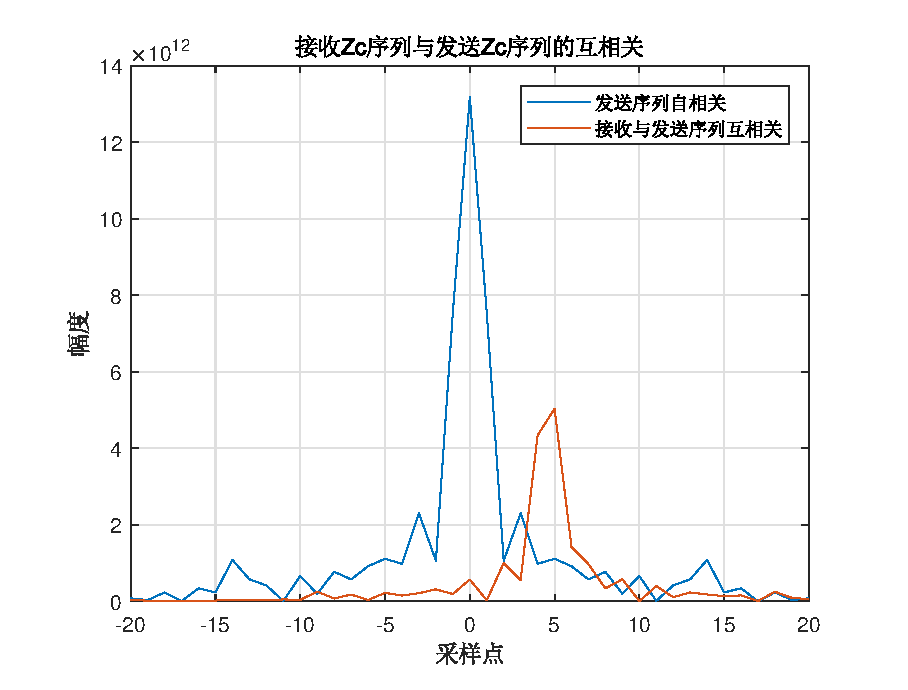
\includegraphics[width = .8\textwidth]{zcco.eps}
	\caption{互相关测试结果}
\end{figure}
\begin{figure}[H]
	\centering
	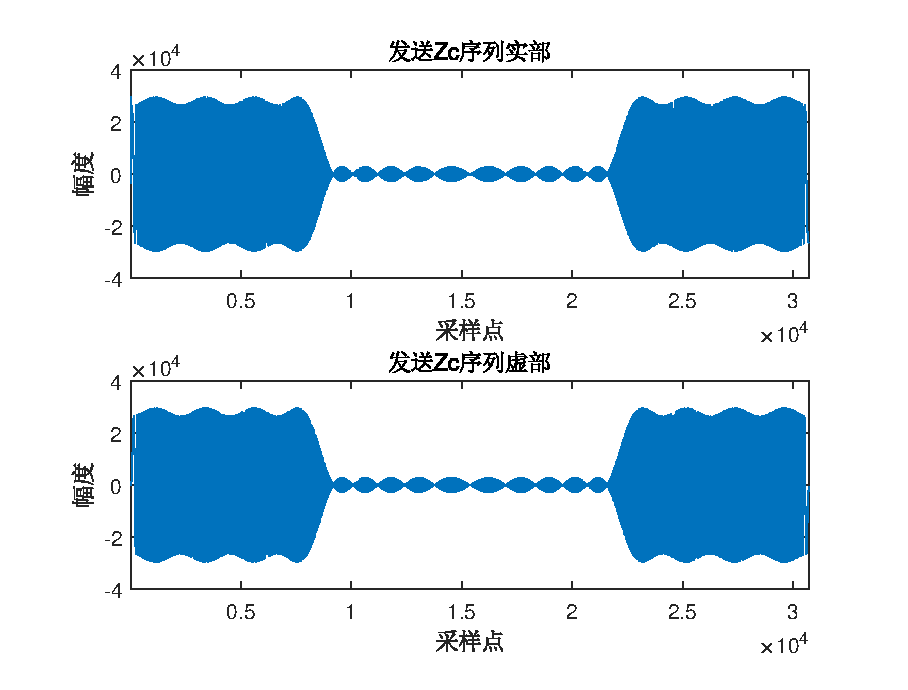
\includegraphics[width = .8\textwidth]{zctx.eps}
	\caption{发送Zc序列时域信号}
\end{figure}
\begin{figure}[H]
	\centering
	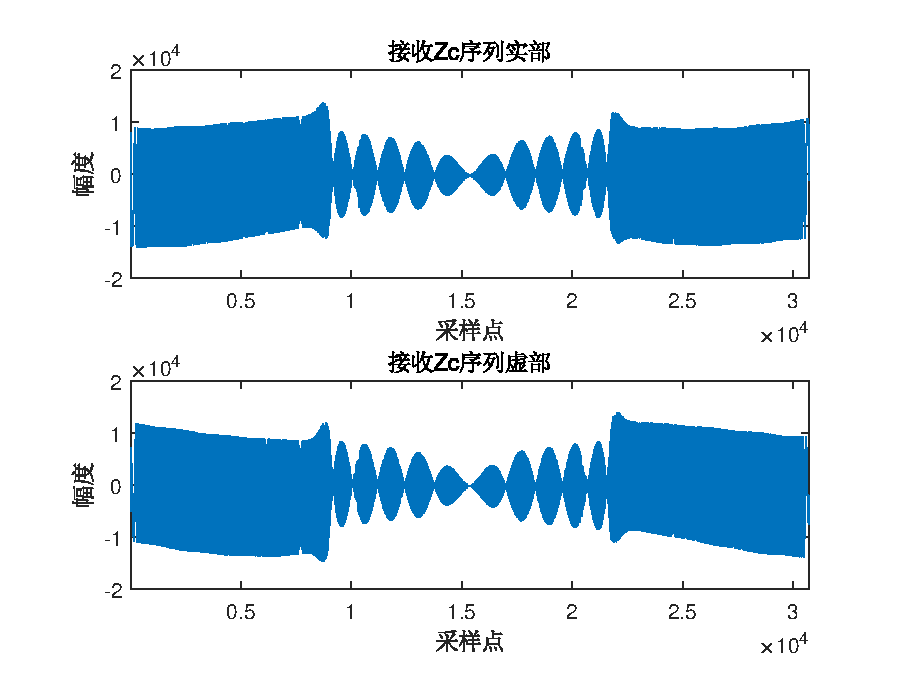
\includegraphics[width = .8\textwidth]{zcrx.eps}
	\caption{接收Zc序列时域信号}
\end{figure}

%===========第二节=================
% \section{关于SVN的问题}
% \begin{figure}[H]
% 	\centering
% 	\includegraphics[width = \textwidth]{svn.png}
% 	\caption{Linux上的错误}
% \end{figure}

%===========第三节=================
% \section{根据PRACH测时延}
% \begin{figure}[H]
% 	\centering
% 	\includegraphics[width = \textwidth]{prach.png}
% 	\caption{时延测试结果}
% \end{figure}

%===========第四节=================
% \section{后续工作}
% 1. 对采集数据进行信道估计;

% 2. 对采集数据进行LTE译码解调;

% 3. 用LDPC编译码替换原单线程系统的Turbo编译码;

% 4. 将带LDPC的系统生成的数据通过底层设备并测试。

%===========下周计划=================
% \section{下阶段计划}
% 1. 继续完成仿真报告

\end{document}
%%%%%%%%%%%%%%%%%%%%%%%这是正文部分的结束%%%%%%%%%%%%